\documentclass{bredelebeamer}

%%%%%%%%%%%%%%%%%%%%%%%%%%%%%%%%%%%%%%%%%%%%%%%%

\title[Programación en MatLAB]{Introducción a la programación con MatLAB}
\subtitle{Módulo 04 - Operaciones vectoriales \textbf{(introducción)}}

\author{- AUTORES - \inst{1}}
\institute[UNIVERSIDAD]
{
  \inst{1}%
  - NOMBRE UNIVERSIDAD - 
  }

\date{AÑO}

\subject{Taller de programación}

\logo{

\includegraphics[scale=0.15]{images/logo.png}
}

%%%%%%%%%%%%%%%%%%%%%%%%%%%%%%%%%%%%%%%%%%%%%%%%%%%%%%%%%%%%%%%%%%%%%
\begin{document}

\begin{frame}
  \titlepage 
\end{frame}

%%%%%%%%%%%%%%%%%%%%%%%%%%%%%%%%%%%%%%%%%%%%%%%%%%%%%%%%%%%%%%%%%%%%%

% Sección de operaciones vectoriales

%%%%%%%%%%%%%%%%%%%%%%%%%%%%%%%%%%%%%%%%%%%%%%%%%%%%%%%%%%%%%%%%%%%%%

\section{Operaciones vectoriales}

\begin{frame}{Tipos de operaciones}
\begin{center}

\includegraphics[scale=0.3]{images/img40.png}
\end{center}
\begin{center}
\textbf{TEMA CORTO *** TEMA CORTO *** TEMA CORTO}
\end{center}
\end{frame}

\begin{frame}{Tipos de operaciones}
\begin{table}[]
\centering
\begin{tabular}{|c|c|}
\hline
\multicolumn{2}{|c|}{a=\{a1,a2,...,an\}, b=\{b1,b2,...,bn\} c=escalar}                                                                           \\ \hline
a+c={[}a1+c a2+c...,an+c{]}                                                                            & Suma de un escalar y un vector          \\ \hline
a*c={[}a1*c a2*c ... an*c{]}                                                                           & Producto de un escalar por un vector    \\ \hline
a + b = {[} a1+b1 a2+b2 ... an+bn{]}                                                                   & Suma de dos vectores                    \\ \hline
\end{tabular}
\end{table}
\end{frame}

\begin{frame}{Tipos de operaciones}
\begin{table}[]
\centering
\begin{tabular}{|c|c|}
\hline
\multicolumn{2}{|c|}{a=\{a1,a2,...,an\}, b=\{b1,b2,...,bn\} c=escalar}                                                                           \\ \hline
a. * b = {[} a1*b1 a2*b2 ... an*bn{]}                                                                  & Producto de dos vectores                \\ \hline
a. / b = {[} a1/b1 a2/b2 ... an/bn{]}                                                                  & Cociente a la derecha de dos vectores   \\ \hline
a.\textasciicircum{}c = {[}a1\textasciicircum{}c a2\textasciicircum{}c ... an\textasciicircum{}c{]}    & Vector elevado a escalar                \\ \hline
c.\textasciicircum{}a = {[}c\textasciicircum{}a1 c\textasciicircum{}a2 ... c\textasciicircum{}an{]}    & Escalar elevado a vector                \\ \hline
a.\textasciicircum{}b = {[}a1\textasciicircum{}b1 a2\textasciicircum{}b2 ... an\textasciicircum{}bn{]} & Vector elevado a vector                 \\ \hline
\end{tabular}
\end{table}
\end{frame}

\begin{frame}{Tipos de operaciones}
\begin{table}[]
\centering
\begin{tabular}{|c|c|}
\hline
\multicolumn{2}{|c|}{a=\{a1,a2,...,an\}, b=\{b1,b2,...,bn\} c=escalar}                                                                           \\ \hline
a. * b = {[} a1*b1 a2*b2 ... an*bn{]}                                                                  & Producto de dos vectores                \\ \hline
a. / b = {[} a1/b1 a2/b2 ... an/bn{]}                                                                  & Cociente a la derecha de dos vectores   \\ \hline
a.\textasciicircum{}c = {[}a1\textasciicircum{}c a2\textasciicircum{}c ... an\textasciicircum{}c{]}    & Vector elevado a escalar                \\ \hline
c.\textasciicircum{}a = {[}c\textasciicircum{}a1 c\textasciicircum{}a2 ... c\textasciicircum{}an{]}    & Escalar elevado a vector                \\ \hline
a.\textasciicircum{}b = {[}a1\textasciicircum{}b1 a2\textasciicircum{}b2 ... an\textasciicircum{}bn{]} & Vector elevado a vector                 \\ \hline
\end{tabular}
\end{table}
\begin{alertblock}{Tener en cuenta}
Los vectores deben ser de igual longitud.
\end{alertblock}
\end{frame}

\begin{frame}{Tipos de operaciones}
\begin{center}
\textbf{Ejemplo de aplicación de a./c}
\end{center}
\begin{center}

\includegraphics[scale=0.6]{images/img41.png}
\end{center}
\end{frame}

\begin{frame}{Ejercicio práctico 5}
\begin{enumerate}
\item Defina la matriz a = [2.3 5.8 9] como una variable
\item Sume 3 a cada elemento en a
\item Defina la matriz b = [5.2 3.14 2] como una variable matlab
\item Sume cada elemento de la matriz a y la matriz b
\item Multiplique cada elemento en a por el correspondiente elemento en b
\item Eleve al cuadrado cada elemento en la matriz a
\item Cree una matriz llamada c de valores igualmente espaciados, desde 0 hasta 10, con un incremento de 1
\item Cree una matriz llamada d de valores igualmente espaciados, desde 0 hasta 10, con un incremento de 2.
\item Use la función linspace para crear una matriz de seis valores igualmente espaciados, desde 10 hasta 20.
\item Use la función logspace para crear una matriz de cinco valores logarítmicamente espaciados entre 10 y 100
\end{enumerate}
\end{frame}

% %%%%%%%%%%%%%%%%%%%%%%%%%%%%%%%%%%%%%%%%%%%%%%%%%%%%%%%%%%%%%%%%%%%%%

% % Sección de consultas

% %%%%%%%%%%%%%%%%%%%%%%%%%%%%%%%%%%%%%%%%%%%%%%%%%%%%%%%%%%%%%%%%%%%%%

% \section{Consultas}
% \begin{frame}{Consultas}
% \begin{center}
% 
\includegraphics[scale=0.3]{images/consultas.png}
% \end{center}
% \end{frame}


% %%%%%%%%%%%%%%%%%%%%%%%%%%%%%%%%%%%%%%%%%%%%%%%%%%%%%%%%%%%%%%%%%%%%%

% % Sección de bibliografía

% %%%%%%%%%%%%%%%%%%%%%%%%%%%%%%%%%%%%%%%%%%%%%%%%%%%%%%%%%%%%%%%%%%%%%

% \section{Bibliografia}

% \begin{frame}{Bibliografía}
% \begin{columns}
% \begin{column}{0.5\textwidth}
% \begin{center}
% 
\includegraphics[scale=0.4]{images/biblio1.png}
% \end{center}
% \end{column}
% \begin{column}{0.5\textwidth}
% \begin{center}
% 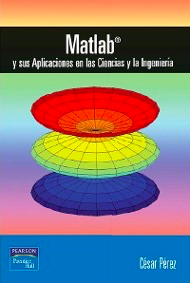
\includegraphics[scale=0.5]{images/biblio2.png}
% \end{center}
% \end{column}
% \end{columns}
% \end{frame}

\end{document}
